% $Id$
%\documentclass[handout]{beamer}
\documentclass{beamer}
\usepackage[utf8]{inputenc}
\usepackage[T1]{fontenc}
\usepackage[swedish,english]{babel}
\usepackage{url}
\usepackage{graphicx}
\usepackage{color}
\usepackage{subfig}
\usepackage{multicol}
\usepackage{csquotes}
\usepackage[natbib,style=alphabetic,maxbibnames=99]{biblatex}
\usepackage{acro}
\addbibresource{msbforts.bib}
\setbeamertemplate{bibliography item}[text]

\DeclareAcronym{isms}
{
  short = ISMS,
  long = Information Security Management Systems,
}
\mode<presentation>{
  \usetheme{Boadilla}
  \usecolortheme{}
  \usefonttheme{professionalfonts}
  \setbeamercovered{transparent}
}
\setbeamerfont{frametitle}{size=\footnotesize}
\setbeamerfont{framesubtitle}{size=\tiny}

\title[Introduction Information Security]{%
  Continuation of the Swedish Civil Contingencies Agency (MSB) 
  methodological support for \ac{isms}\\
  MSB:s metodstöd
}
\author{Carina Bengtsson, Daniel Bosk and Lennart Franked\footnote{%
  Detta verk är tillgängliggjort under licensen Creative Commons 
  Erkännande-DelaLika 2.5 Sverige (CC BY-SA 2.5 SE).
	För att se en sammanfattning och kopia av licenstexten besök URL 
	\url{http://creativecommons.org/licenses/by-sa/2.5/se/}.
}}
\institute[MIUN ITM]{%
  Department of Informationsystems and Technologies\\
  Mid Sweden University,
  Sundsvall.
}
\date{\today}

\AtBeginSection[]{%
  \begin{frame}<beamer>{Översikt}
    \begin{multicols}{2}
      \tableofcontents[currentsection]
    \end{multicols}
  \end{frame}
}

\begin{document}

\begin{frame}
  \titlepage{}
\end{frame}

\begin{frame}{Overview}
  \begin{multicols}{2}
    \tableofcontents
  \end{multicols}
	% You might wish to add the option [pausesections]
\end{frame}

% Since this a solution template for a generic talk, very little can
% be said about how it should be structured. However, the talk length
% of between 15min and 45min and the theme suggest that you stick to
% the following rules:  

% - Exactly two or three sections (other than the summary).
% - At *most* three subsections per section.
% - Talk about 30s to 2min per frame. So there should be between about
%   15 and 30 frames, all told.


\section{Analysis}

\subsection{Organisational Analyses}

\begin{frame}{What needs protecting?}
  \begin{itemize}
    \item What informational assets do we have, and how much are they worth
      protecting?
    \item Should lead to a structured list over
      \begin{itemize}
        \item what informational assets there are,,
        \item what requirements and expectations they have, and
        \item the worth of each asset.
      \end{itemize}
  \end{itemize}
\end{frame}

\begin{frame}{Finding the informational assets}
  \begin{itemize}
    \item Previous process mappings?
    \item Department wise?
    \item IT-system?
    \item Project?
    \item Processes?
    \item By function?
  \end{itemize}
\end{frame}

\begin{frame}{MSB:s suggestion on a classification model}
  \begin{figure}
    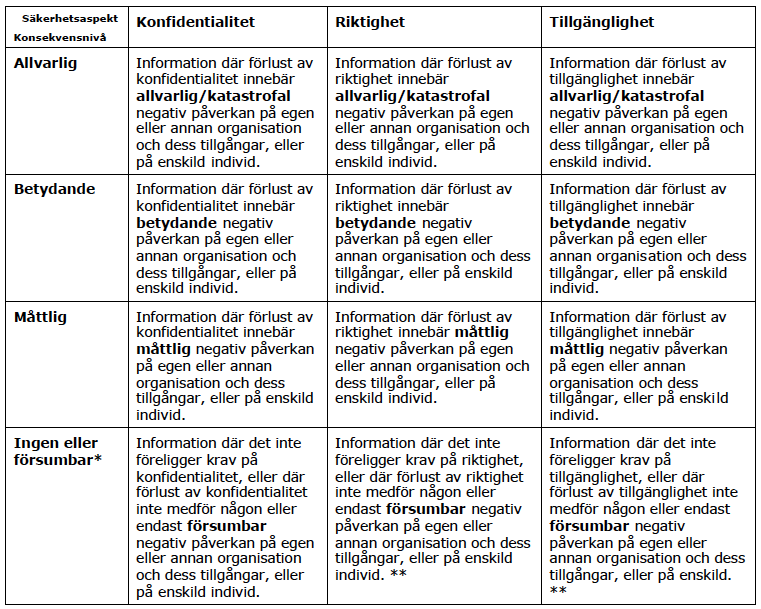
\includegraphics[height=0.7\textheight]{msb-klassificering.png}
    \caption{MSB:s suggestion on a classification model.}
  \end{figure}
\end{frame}

\begin{frame}{University's adaptation of a classification model.}
  \begin{figure}
    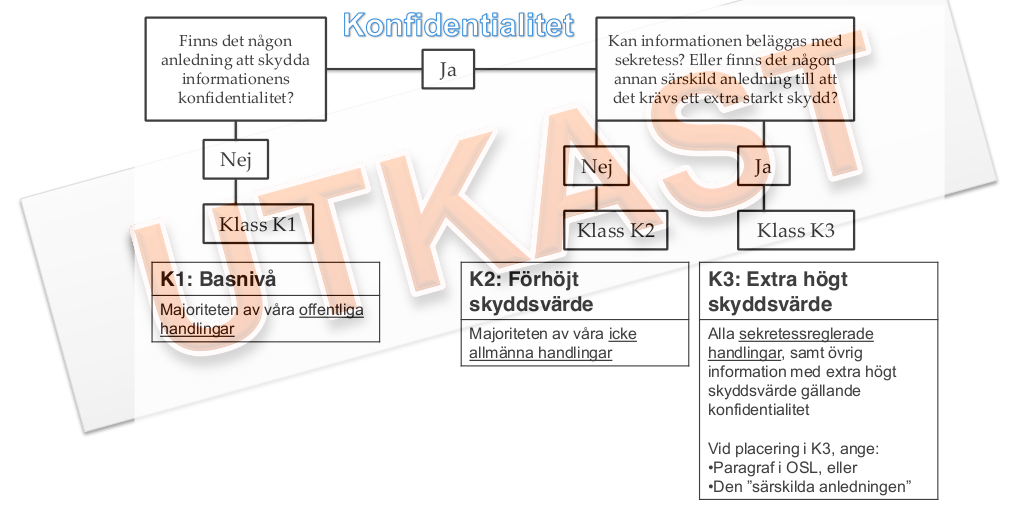
\includegraphics[width=\textwidth]{miun-klassificering.png}
    \caption{University's adaptation of a classification model from the
      confidentiality perspective.}
  \end{figure}
\end{frame}

\subsection{Risk analysis}

\begin{frame}{Risk analysis}
  \begin{itemize}
    \item Used to adapt the protection based on the assets of the organisation.
    \item Generate a list over
      \begin{itemize}
        \item existing threats,
        \item consequences of the threats, and
        \item suggestions for risk management.
      \end{itemize}
  \end{itemize}
\end{frame}

\begin{frame}{Risk matrix}
  \begin{figure}
    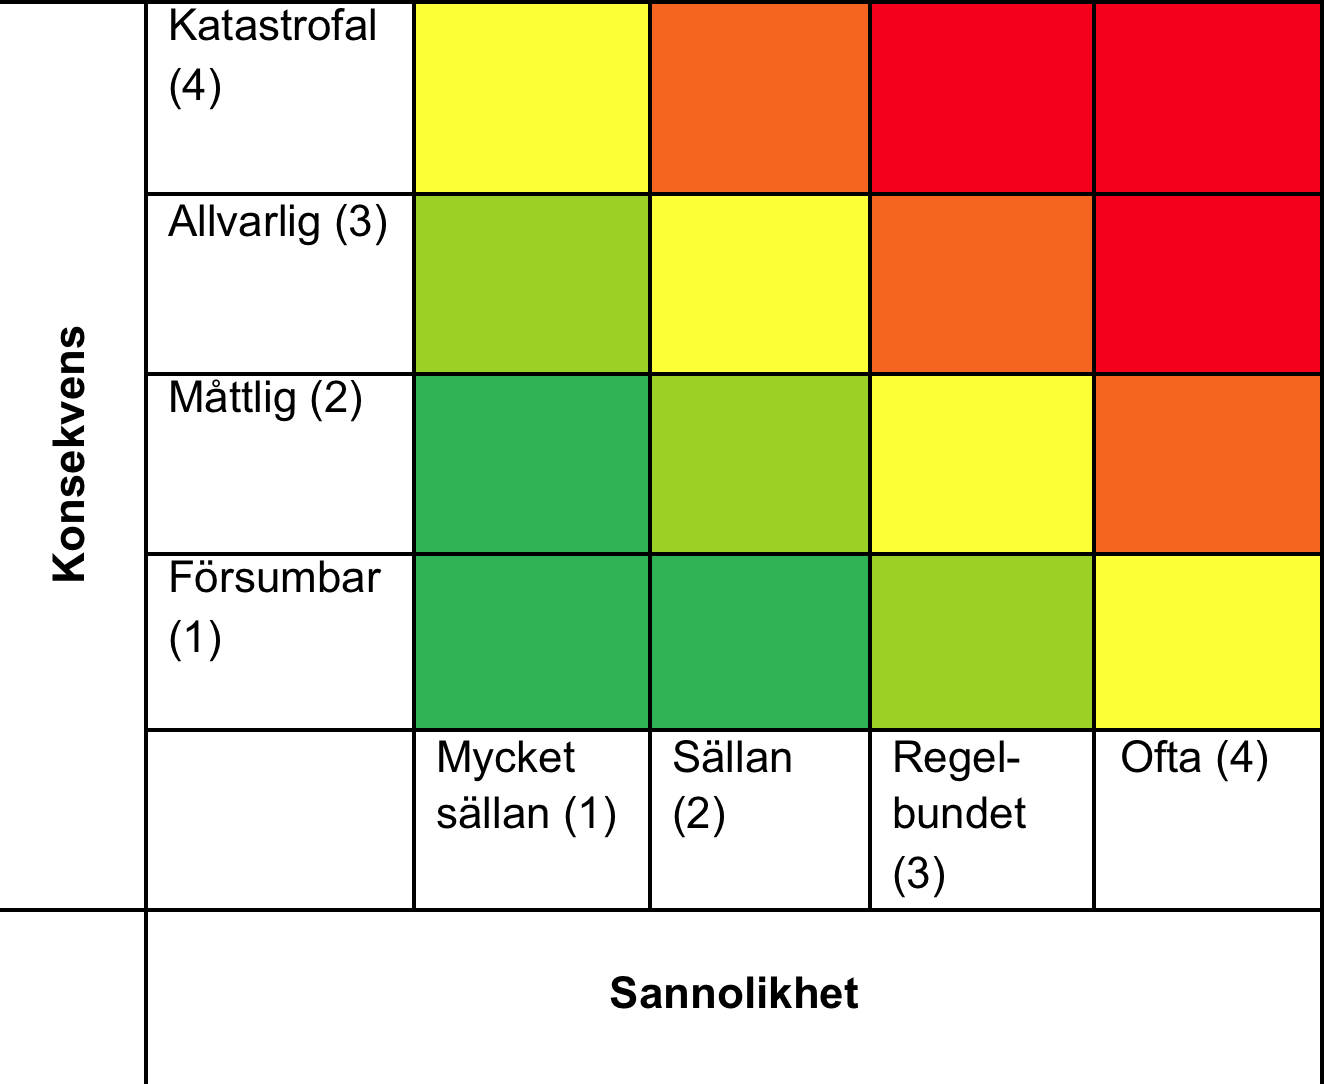
\includegraphics[height=0.7\textheight]{riskmatris.png}
    \caption{A risk matrix.}
  \end{figure}
\end{frame}

\begin{frame}{Formal methods?}
  \begin{itemize}
    \item There are a lot of research done regarding how to perform risk
      analysis.
    \item They can, however be difficult to use.
  \end{itemize}
\end{frame}

\section{Gap Analysis}

\subsection{What is a gap analysis?}

\begin{frame}
  \begin{itemize}
    \item Analyses the gap between the organisations current information
      security, and its set goals.
    \item The methodological support from MSB uses the norm described in ISO
      27002, instead of the goal of the organisation.
    \item The following result will therefore show how the organisation stands
      in comparison to the expectations in ISO 27002.
  \end{itemize}
\end{frame}

\begin{frame}
  Investigates what security measures that
  \begin{itemize}
    \item exists and working,
    \item exists but doesn't work,
    \item doesn't exist,
    \item isn't needed.
  \end{itemize}
\end{frame}

\begin{frame}{When is a gap analysis performed?}
  \begin{itemize}
    \item If you want to establish an \ac{isms}\@.
    \item If you want to measure, audit or verify the information security level
      of the organisation.
    \item If you want to establish requirements on your information security
      level.
  \end{itemize}
\end{frame}

\subsection{How should it be done?}

\begin{frame}{Requirements for performing a gap analysis}
  The project leader of the analysis task must
  \begin{itemize}
    \item know the organisations need and requirements,
    \item know any existing governance documents regarding the security work in
      the organisation,
    \item have a good knowledge and understanding of the norms in the standard.
  \end{itemize}
\end{frame}

\begin{frame}
  \begin{itemize}
    \item There must exist a clear decision that a gap analysis should be
      performed,
    \item Otherwise there must exist a clear mandate to be able to make this call.
    \item As a support, use MSB:s checklist for gap analysis~\cite{MSB2011gb}.
  \end{itemize}
\end{frame}

\subsection{The checklist}

\begin{frame}
  \begin{itemize}
    \item Based on ISO 27002.
    \item Contains 133 security measures.
    \item Each security measure have one or several questions that helps set the
      level, based on a scale between 0-3.
    \item Each security measure belongs to a section.
    \item Each section belongs to a chapter (area/field).
    \item There are in total 11 chapters.
  \end{itemize}
\end{frame}

\begin{frame}{The Checklist}
  \begin{itemize}
    \item Out of a total of a 133 security measures, 62 (55) are deemed critical.
    \item The critical measures is used as a lowest acceptable level for
      the information security.
  \end{itemize}
\end{frame}

\subsection{Practical Implementation}

\begin{frame}{Who?}
  \begin{itemize}
    \item Analysis leader.
    \item Experts in the organisation that is most suitable to answer each field
      in the checklist.
    \item Doesn't necessarily need to be the managers.
  \end{itemize}
\end{frame}

\begin{frame}{Practical Implementation}
  \begin{itemize}
    \item Book a meeting with the experts.
    \item Send the questions to the experts in advance.
    \item At the meeting: Work through all the questions.
  \end{itemize}
\end{frame}

\begin{frame}{Level setting questions}
  \begin{figure}
    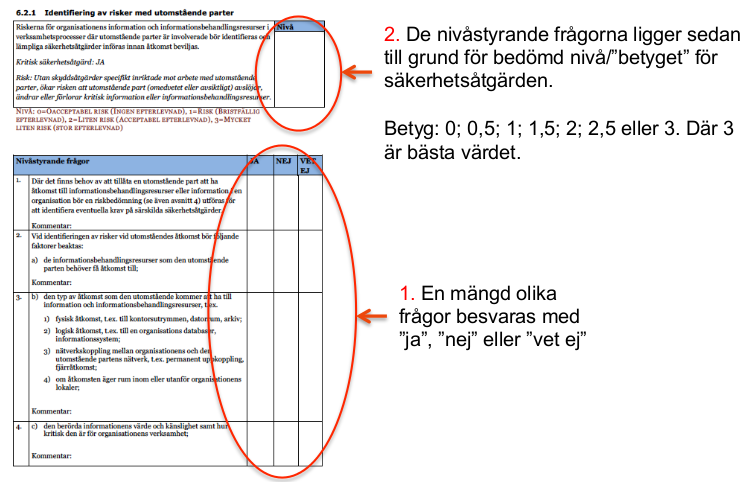
\includegraphics[height=0.7\textheight]{gap-nivafragor.png}
    \caption{Level setting questions that gives an estimate value of security
      measures.}
  \end{figure}
\end{frame}

\begin{frame}{Summary of subsection}
  \begin{figure}
    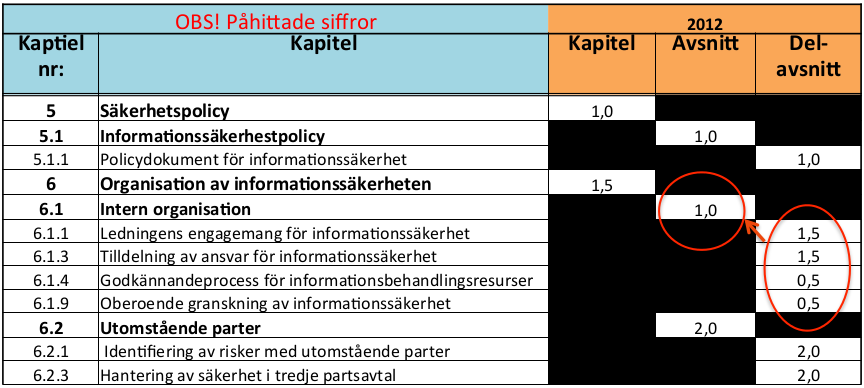
\includegraphics[width=\textwidth]{gap-sammanstallning.png}
    \caption{The grade of the section is based upon the grades of each subsection}
  \end{figure}
\end{frame}

\begin{frame}{Summary of section}
  \begin{figure}
    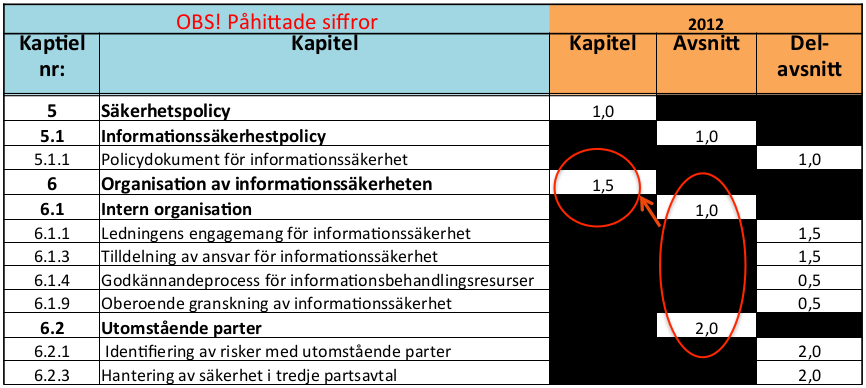
\includegraphics[width=\textwidth]{gap-kapitel.png}
    \caption{The grade of the chapter is based upon the grades of each section.}
  \end{figure}
\end{frame}

\begin{frame}{Summarizing the grades.}
  \begin{figure}
    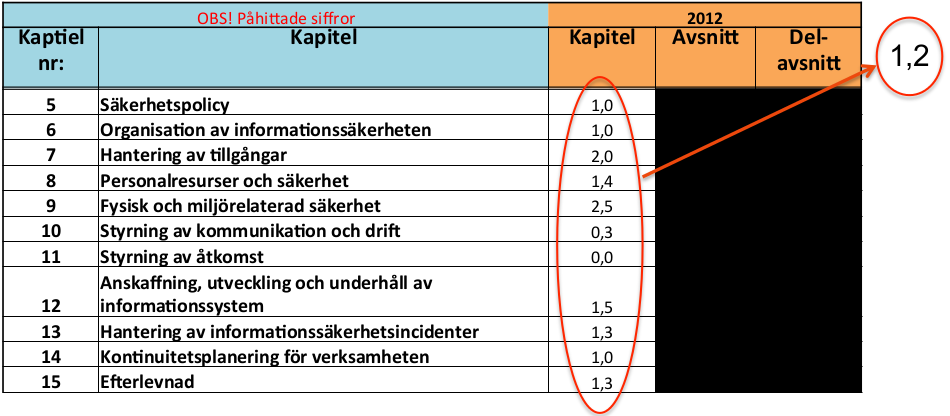
\includegraphics[width=\textwidth]{gap-betyg.png}
    \caption{The total grade is based upon the grades of each chapter.}
  \end{figure}
\end{frame}

\subsection{Overview of ISO 27002}

\begin{frame}{ISO 27002}
  \begin{enumerate}
    \item Security Policy
    \item Organisation surrounding information security.
    \item Management of assets.
    \item Human resources and security
    \item Physical and environmental security
    \item Control of communication and management.
    \item Access control.
    \item Acquiring, developing and maintaining information systems.
    \item Managing information security incidents.
    \item Contingency planning for the organisation.
    \item Compliance.
  \end{enumerate}
\end{frame}

\begin{frame}{ISO 27002}{Security Policy}
  \begin{itemize}
    \item What is the directional intent for the organisation in regards to
      information security.
    \item How should this be achieved.
    \item Short explanation of terminology
    \item How will the responsibility be divided.
    \item Legal and internal requirements should be taken into account.
  \end{itemize}
\end{frame}

\begin{frame}{ISO 27002}{Organisation surrounding information security}
  \begin{itemize}
    \item Should exist a framework within the organisation that is controlling
      the information security.
    \item Decisions need to be taken regarding governance documents.
    \item Clearly stated how responsibilities are divided.
    \item Contains six critical security measures.
  \end{itemize}
\end{frame}

\begin{frame}{ISO 27002}{Management of assets}
  \begin{itemize}
    \item Ensuring that the assets in the organisation should have a suitable
      protection.
    \item Contains two critical security measures: List of assets and guidelines
      for classifying assets.
  \end{itemize}
\end{frame}

\begin{frame}{ISO 27002}{Human resources and security}
  \begin{itemize}
    \item What to take into account before, during and after employment within
      the organisation. 
    \item Background checks, in house training, how to handle permissions when
      an employment has been ended.
    \item Contains three critical security measures.
  \end{itemize}
\end{frame}

\begin{frame}{ISO 27002}{Physical and environmental security}
  \begin{itemize}
    \item To prevent unauthorized access.
    \item Reduce the risk of damage on informational assets.
    \item Contains four critical security measures.
  \end{itemize}
\end{frame}

\begin{frame}{ISO 27002}{Control of communication and management}
  \begin{itemize}
    \item Resources that are managing information should have a safe and reliable operation.
    \item Clearly state the responsibilities and the documentation for this.
    \item Have 14 critical security measures.
  \end{itemize}
\end{frame}

\begin{frame}{ISO 27002}{Access Control}
  \begin{itemize}
    \item Access to the system should be controlled through the organisational
      and security requirements.
    \item Contains ten critical security measures.
  \end{itemize}
\end{frame}

\begin{frame}{ISO 27002}{Acquiring, developing and maintaining information systems}
  \begin{itemize}
    \item Ensure that new and existing information systems are keeping a high
      security level.
    \item Contains seven critical security measures.
  \end{itemize}
\end{frame}

\begin{frame}{ISO 27002}{Managing information security incidents}
  \begin{itemize}
    \item Security incidents should be handled.
    \item Reduce the risk of an incident happening again.
    \item Contains two critical security measures.
  \end{itemize}
\end{frame}

\begin{frame}{ISO 27002}{Contingency planning for the organisation}
  \begin{itemize}
    \item Prevent disruptions in the organisation.
    \item Learn how to deal with disruptions.
    \item Contains three critical security measures.
  \end{itemize}
\end{frame}

\begin{frame}{ISO 27002}{Compliance}
  \begin{itemize}
    \item Ensures that the organisation comply to the external and internal
      requirements that exist in regards to information security.
    \item Contains three critical security measures.
  \end{itemize}
\end{frame}

\subsection{Results}

\begin{frame}{Result of the gap analysis}
  \begin{itemize}
    \item Which security measurements are implemented?
    \item What are the scope and quality on the implemented measurements?
    \item What weaknesses and strength are there on the implemented
      measurements?
    \item What is the next step\@?
  \end{itemize}
\end{frame}

\begin{frame}{Report}
  \begin{itemize}
    \item How well have the work been done?
    \item What are the input values that have been used?
    \item What is the result of the analysis?
    \item Summary of the entire work.
    \item Suggestions on how to continue.
  \end{itemize}
\end{frame}

\section{Establish}

\subsection{Measurement}

\begin{frame}{How to choose the security measurement}
  \begin{figure}
    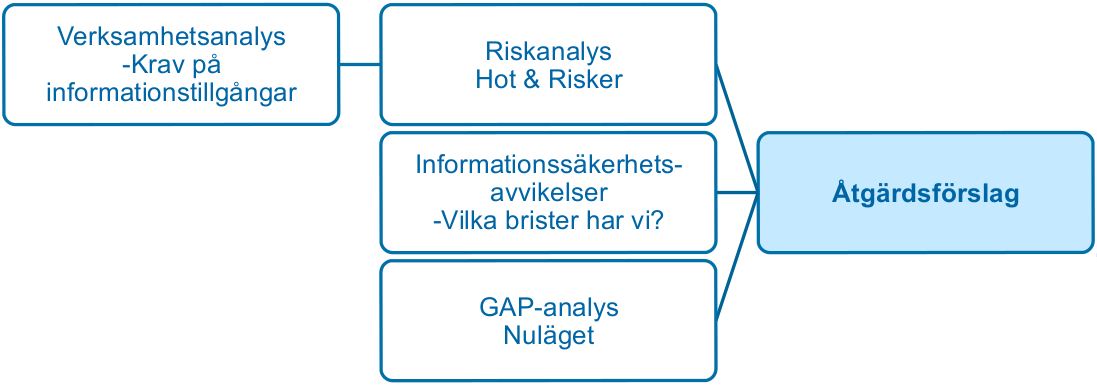
\includegraphics[width=\textwidth]{msb-atgarder.png}
    \caption{Choosing security measures.}
  \end{figure}
\end{frame}

\begin{frame}{Selecting the measurements}
  \begin{description}
    \item[Best practice] Based upon different security measures listed in ISO
      27002.
    \item[Risk analysis] Tailored security measures based solely on
      organisations need.
  \end{description}
  \begin{itemize}
    \item Base analysis -- the need for protection.
    \item Will the protection have wished effect?
    \item Focus on \emph{if} they should be implemented, not \emph{how}.
  \end{itemize}
\end{frame}
\begin{frame}{Type of measurements}
  \begin{itemize}
    \item Governance documents.
    \item Analysis, monitoring.
    \item Technical protection.
    \item Education.
    \item Processes.
  \end{itemize}
\end{frame}

\subsection{Processes}
\begin{frame}{Develop security processes}
  \begin{itemize}
    \item Collection of activities that manages a defined need.
    \item Integrate with existing processes.
    \item For example \ac{isms}.
    \item Examples: Information security classification, access control.
  \end{itemize}
\end{frame}
\begin{frame}{Developing processes}
  \begin{itemize}
    \item Wide competence.
    \item Representatives from the entire (affected parts) organisation.
    \item Makes it easier to coordinate with existing processes.
  \end{itemize}
\end{frame}

\subsection{Governance documents}
\begin{frame}{Develop governance documents}
  \begin{itemize}
    \item Start with one policy, what is the directional intent of the organisation.
    \item Identify existing documents: revise, revoke, introduce new.
    \item Adapt based on the current document structure.
  \end{itemize}
\end{frame}
\begin{frame}{Develop governance documents}
  Don't forget
  \begin{itemize}
    \item version control,
    \item document owner,
    \item decision date,
    \item who took the decision.
  \end{itemize}
  They should be written in such a way that everyone can understand them
\end{frame}

\section{Implementation}
\begin{frame}{Implementation}
  \begin{itemize}
    \item At this stage security processes are formed and decisions have been
      made for taking security measures.
    \item Can be done in project form, or just incorporated into the regular work load.
  \end{itemize}
\end{frame}

\subsection{Plan the implementation}
\begin{frame}{Plan the implementation}
  \begin{itemize}
    \item Should something be prioritized?
    \item Do some implementation measures dependend on others?
    \item What can be constructed, and what can be procured?
    \item Need a time plan, and ensure everyone is aware that the work will
      start.
  \end{itemize}
\end{frame}

\subsection{Construct and procure}
\begin{frame}{Construct and procure}
  \begin{description}
    \item[Construct] The organisation to in-house development.
    \item[Procure] The organisation procures solutions.
  \end{description}
  \begin{figure}
    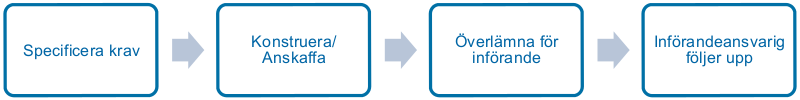
\includegraphics[width=\textwidth]{infora.png}
    \caption{Process to construct and procure.}
  \end{figure}
\end{frame}
\begin{frame}{Defining requirements}
  \begin{itemize}
    \item Important clearly have stated what requirements exist.
    \item IT-department are unaware of how much the information they are
      managing is worth protecting -- Need to be specified.
    \item Think about usability to ensure that the organisation do not
      circumvent the measures.
  \end{itemize}
\end{frame}

\subsection{Implement}
\begin{frame}{Implement}
  \begin{itemize}
    \item One coordinator.
    \item Multiple persons responsible for the practical.
    \item The work is carried out in groups: Include area managers that are
      affected by the security measures.
  \end{itemize}
\end{frame}
\begin{frame}{Groups responsible for implementing the security measures}
  Focus on:
  \begin{itemize}
    \item Representation of the entire organisation.
    \item Do the employees need training?
      They need to be able to use and understand the security measures.
    \item Who should manage the security measures?
      There is a need for a management plan.
    \item Ensuring that the organisation will embrace the measures.
  \end{itemize}
\end{frame}
\begin{frame}{Changing the behaviour}
  \begin{itemize}
    \item Many security measures needs a change in the behaviour to work.
    \item Communicate and explain \emph{why} -- Make sure the explanation is
      targeted.
  \end{itemize}
\end{frame}


\section{Follow Up}

\subsection{Monitor}
\begin{frame}{Monitor}
  \begin{itemize}
    \item Should be done continuously in different levels in the organisation.
    \item Will be used as a base for further analysis of the security measure,
      and for presenting to the top management.
  \end{itemize}
\end{frame}
\begin{frame}{Evaluation}
  Ensure that the right conditions exist for evaluation:
  \begin{itemize}
    \item Effect of \ac{isms}\@: Are there sufficient measurements in place towards the current threats?
    \item Effect of the security measurements: Have they been implemented?
    \item How have the informational assets been affected: Have the secrecy become greater?
  \end{itemize}
\end{frame}
\begin{frame}{Incident management}
  \begin{itemize}
    \item A part of the monitoring, which purpose is to discover new threats.
    \item Discover any shortcomings in the measurements taken for previously
      known threats.
    \item This also includes fixing these shortcomings.
  \end{itemize}
  \begin{figure}
    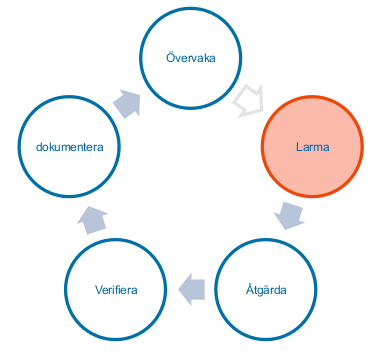
\includegraphics[height=0.4\textheight]{overvakning.png}
    \caption{Cycle for monitoring and incident management.}
  \end{figure}
\end{frame}

\subsection{Review}
\begin{frame}{Review}
  \begin{itemize}
    \item A deeper analysis of the result from the monitoring.
    \item Part of the recurring organisational follow-ups, for example internal
      revision.
    \item Use the information from the monitoring as base.
    \item Is the \ac{isms} working\@?
  \end{itemize}
\end{frame}
\begin{frame}{Audit requirement}
  \begin{itemize}
    \item ISO 27001: the top management must ensure this is done -- and should
      take part of the result.
    \item How?
      \begin{itemize}
        \item Use ISO 27001 \ac{isms}\@.
        \item Use ISO 27002 for the security measures.
      \end{itemize}
    \item Who?
      Independent auditor with the support from those who are responsible for
      the \ac{isms}.
  \end{itemize}
\end{frame}

\subsection{Top Management Review}
\begin{frame}{Top Management Review}
  \begin{itemize}
    \item The top management are responsible for the entire organisation.
    \item It is important that they understand the result of the audit.
    \item Recommended to have a yearly review of the information security.
  \end{itemize}
\end{frame}
\begin{frame}{Top Management Review}
  \begin{itemize}
    \item Should be given by the person responsible for the information
      security, along with the experts from the GAP-analysis.
    \item Should be done yearly.
  \end{itemize}
\end{frame}
\begin{frame}{\insertsubsectionhead}
  \begin{itemize}
    \item Should include the result of the audits, weaknesses and threats that
      haven't been fully covered from the last risk assessment.
    \item Should result in decisions regarding how to improve the result of the
      \ac{isms}, update of risk assessment and risk treatment plan.
  \end{itemize}
\end{frame}


\section{Improve}

\subsection{Improve \ac{isms} and the protection}
\begin{frame}{\insertsubsectionhead}
  \begin{itemize}
    \item Use the result from follow-ups and the top management review.
    \item Recommended that the process is done in a structured way, PDCA
    \item Standardise: Establish the measures in the governance documents, ensure
      that they are implemented correctly.
  \end{itemize}
\end{frame}

\subsection{Communicate the improvements}
\begin{frame}{\insertsubsectionhead}
  Try to create an interest that ensures that the
  \begin{itemize}
    \item employees \emph{will learn},
    \item get a \emph{positive} attitude towards information security,
    \item have an \emph{intention} to work towards improving the information
      security,
    \item and changes their behavior.
  \end{itemize}
\end{frame}

%%%%%%%%%%%%%%%%%%%%%%

\begin{frame}[allowframebreaks]{Referenser}
	\small
  \printbibliography{}
\end{frame}

\end{document}

